\documentclass[10pt,letterpaper]{article}

\usepackage{cogsci}
\usepackage{pslatex}
\usepackage{apacite2}
\usepackage{amsmath}
% \usepackage{hyperref}
\usepackage{graphicx}

\DeclareMathOperator*{\argmax}{arg\,max}

\title{Modeling the dynamics of classroom education using teaching games}
 
\author{{\large \bf Michael C. Frank} \\
  \texttt{mcfrank@stanford.edu} \\
  Department of Psychology\\
  Stanford University}


\begin{document}

\maketitle

\begin{abstract}
What makes a good teacher? We consider the idea that a good teacher is a good communicator, using models of optimal communication to explore the dynamics of classroom teaching. We explore the challenges of communicating to a heterogenous audience. Our model describes teaching as choosing examples of a concept to present to students in order to maximize their information gain. A number of results emerge naturally from this model, including (1) decreases in performance with increases in class size, (2) increases in performance based on grouping (``tracking'') students by abilities, and (3) the value of formative evaluation to enhance teachers' knowledge of student ability. 

\textbf{Keywords:} 
Bayesian modeling; teaching; education; communication.
\end{abstract}

\section{Introduction}

What makes a good teacher? Intuitively, a good teacher is a good communicator, choosing explanations and examples that allow students to learn effectively. In our current work I explore this parallel between teaching and communication. I examine how variability in both the size and the knowledgeability of teachers' audience affects communication strategies via a formal model of optimal classroom teaching.  

Recent formal work using probabilistic models has developed the parallel between teaching and communication. \citeA{shafto2008} described a model of teaching to a single student, in which teacher and learner reason recursively about one another's intentions. In this model, the teacher's goal is to choose an example or set of examples to allow a learner to acquire a concept (say, a rectangle in the coordinate plane). The learner then reasons about the examples that the teacher has chosen, given that the teacher has chosen them with her in mind (e.g. in order to maximize her learning). This recursive form---teacher chooses examples to maximize learning, learner considers teacher's choice---leads to much stronger inferences than in scenarios where the learner does not reason about the teacher \cite{shafto2012}.

Though some models of this type employ very deep recursion, depth is not necessary for a good fit to human behavior. In a recent model of pragmatic communication, \citeA{frank2012} developed a version of this framework that described speakers as choosing their words to convey maximal information to a naive listener who literally interprets their words). The spirit of this framework guides the current work: Teachers are modeled as speakers who consider the beliefs of a group of students when choosing what example to present. 

The goal of this work is to create a simple model of the dynamics of classroom teaching. The inspiration comes from ``ideal observer'' analyses of perception that provide a baseline model with which to assess human performance \cite{geisler2003,frank2013}. Similarly, a model of classroom education
could provide a tool for reasoning about the causal factors involved in student outcomes. Further down the road, to the extent its predictions match human behavior they could be a guide for future research or even---in combination with a model of the cost of interventions---to promote effective decision-making. 

Many questions about classroom education are both foundational and highly controversial. For example, do larger classes produce worse learning outcomes for students \cite{glass1979,slavin1989}? Does separating students by ability produce better learning \cite{slavin1987,wheelock1992}? Is it better to spend class time testing students' initial performance in order to customize curriculum, or is it better to standardize materials \cite{fuchs1986}? The hope is that models like the one we describe here will provide a guide to reasoning about these issues.

The fundamental unit of analysis is a teaching game. In this game, a teacher attempts to guide a group of students to discover a simple concept, in our case the weight of a biased coin. The challenge for the teacher is that he\footnote{For clarity (but hopefully without implication of bias), I adopt a gendered pronoun to describe the teacher.} can only convey this concept by the use of examples; in our case these examples are outcomes of flipping the coin. What examples should the teacher choose? If his students are perfectly unbiased, his examples should follow the overall distribution of the coin. So for a fair coin he should provide e.g., $HTHT$. But what if he knows that his students believe the coin to be biased in favor of heads (say $C=.25$), while it is actually biased somewhat in favor of tails ($C=.75$). What sequence should he show then? Intuitively, his choice might be more likely to skew towards sequences with more heads than the actual proportion, in order to counteract the students' bias.

Our model formalizes this intuition using a probabilistic framework in which students are described as optimal learners given some prior beliefs and the teacher makes his decisions based on knowledge about these learners. The initial Model section presents computational details, and the simulations section provides some results using the model. Without modification or fitting, the model reproduces a range of intuitive phenomena including the influence of class size and heterogeneity on student performance, and the results of grouping students into classes by ability (``tracking''). 

\section{Model}

In our teaching games, we assume that a teacher $T$ attempts to provide information to students $S = {s_1 ... s_n}$. The teacher conveys information by choosing examples $E = {e_1 ... e_m}$ to illustrate an underlying concept $C$, based on some estimate of the students' prior knowledge and abilities $\hat{S} = {\hat{s_1} ... \hat{s_m}}$. Learners in turn attempt to recover $C$ with maximal fidelity. The teacher's payoff is determined by a test, administered to each of the learners. 

We consider a very simple form of this sort of game in which the teacher chooses a single example of $C$ to inform the students.\footnote{All code available at \url{http://github.com/mcfrank/teaching}.}
 In addition, we assume that the teacher has perfect knowledge of students' initial and final state for purposes of planning her moves. These assumptions can of course be relaxed in future work.

We also begin by considering the teaching of a very simple concept: the weight on a coin (a single Bernoulli variable). The exact weight on this coin is unknown, but both teacher and student maintain a distribution of beliefs about the coin weight. The teacher wishes to modify the student's belief distribution so that it is similar to her own. In order to do so she can make exactly one choice, which is whether the example $e$ that she shows should be heads, notated $H$ (which we assume by convention is valued 0), or tails, notated $T$ (similarly, valued 1). Based on this example, the students will rationally update their beliefs, and their new beliefs will be evaluated with respect to their initial state to determine whether they have learned.

\subsection{Students}

\begin{figure}[t]
\begin{center}
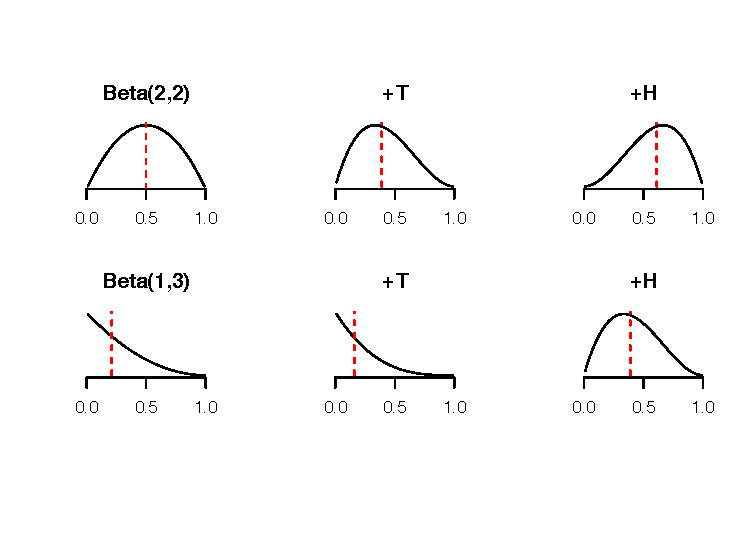
\includegraphics[width=3.25in]{figures/students2.pdf}
\end{center}
\caption{\label{fig:students} Two examples of the Beta-Bernoulli distribution with different priors and patterns of evidence. Black curves show probability distribution with a given prior (left column) and after observing a single head or tail (middle and right columns). Red lines show posterior mean.}
\end{figure}

We model the student here as a Bayesian (optimal) estimator of the target Bernoulli distribution, using a conjugate Beta-Bernoulli distribution. This model is very convenient: the form of the prior distribution is $Beta(\alpha,\beta)$, and the form of the posterior can be written $Beta(\alpha+x,\beta+y)$ where $x$ and $y$ represent the number of heads and tails observed in the data. In this sense, if $x$ and $y$ are the \emph{counts} of observed data, then $\alpha$ and $\beta$ can be referred to as \emph{pseudo-counts}.

This formulation also gives us a way to model both the student's abilities and their prior knowledge about the situation. Consider the example Beta-Bernoulli distributions shown in Figure \ref{fig:students}. Symmetric priors of $\alpha=\beta=2$ lead to a bias that the target coin weight is around .5, while $\alpha=1, \beta=3$ leads to a bias towards lower values. 

Under this formulation, the prior controls both the speed at which a student will learn and their overall bias. For example, as $\alpha$ and $\beta$ both go towards 0, the student's estimate converges to a maximum-likelihood estimate based on the observed data alone. In contrast, as $\alpha$ and $\beta$ both get larger, the student makes less and less use of the data and is more and more reliant on the shape of the prior distribution. The relative weights of $\alpha$ and $\beta$ control the student's mean estimate---greater pseudo-counts on one or the other will lead to greater bias to believe that the correct parameter is lower or higher. 

As described below, students' learning rate is less important than their bias. For this reason, we use an alternative parameterization of the Beta-Bernoulli distribution, in terms of shape $\mu$ and scale $\nu$, where

\begin{eqnarray}
\mu &=& \alpha / \alpha + \beta \\
\nu &=& \alpha + \beta
\end{eqnarray}

\noindent $\mu$ directly controls the mean of the distribution, while $\nu$ captures the strength of the belief. For example, in Figure \ref{fig:students}, $\mu=.5$ for all three prior distributions (left column), while $\nu = 1$, 2, and 4, respectively.

\subsection{Evaluation}

We compute the information gain from the teacher's particular example via information theory. We notate the Beta distribution of the teacher's beliefs as $B_T = Beta(\alpha_T,\beta_T)$, and similarly the student's Beta distributions before and after seeing the teacher's example as $B_{S}$ and $B_{S+e}$ respectively. This allows us to compute the Kullback-Leibler divergence \cite{cover2012} between student and teacher, both before and after seeing example $e$. The divergence between these two quantities is the information gain due to the example:

\begin{equation}
\label{eq:ig}
IG(e) = D_{KL} ( B_{S})||B_T )  - D_{KL} ( B_{S+e} ||B_T ) 
\end{equation}

\noindent where the divergence measure is computed

\begin{equation}
\label{eq:dkl}
\begin{split}
D_{KL} ( B_{S})||B_T )  = & \log( \frac{B(\alpha_{S},\beta_{S})}{B(\alpha_{T},\beta_{T})}) + \\
& (\alpha_T - \alpha_S) \psi (\alpha_T) + \\ 
& (\beta_T - \beta_S) \psi (\beta_T) + \\
& (\alpha_T - \alpha_S + \beta_T - \beta_S) \psi (\alpha_T + \beta_T). \\
\end{split}
\end{equation}

\noindent Information gain will be positive when $B_{S+e}$ is closer to the target distribution than $B_S$.

An interesting property of information gain, when defined in this way, is that it is insensitive to the scale parameter of the students' prior estimate. If Equation \ref{eq:dkl} is substituted into Equation \ref{eq:ig}, and we assume that $e=H$, Equation \ref{eq:ig} reduces to

\begin{equation}
IG(e) = \log(\frac{\alpha_S + \beta_S}{\alpha_S}) + \psi (\alpha_T) + \psi (\alpha_T + \beta_T).
\end{equation}

\noindent Only the first of these terms depends at all on the student's knowledge. That term ($\log(\frac{\alpha_S + \beta_S}{\alpha_S})$) depends on the ratio of $\alpha_S$ to $\beta_S$ but not their absolute values. Thus, only the relative size of $\alpha$ and $\beta$ (captured via the $\mu$ parameter) matters. In practical terms, this result implies that we need only vary the $\mu$ parameer for individual students in our simulations.

\subsection{Teachers}

The teacher is assumed to choose between possible examples in the set $E$ (in our case, just $H$ or $T$) so as to maximize the average information gain across students. Thus their expected information gain is the information gain due to the best example that they could show:

\begin{equation}
E[IG] = \argmax_e {IG(e)}.
\end{equation}

\noindent Note that this formulation assumes that they have perfect knowledge of the students both before and after an example and can mentally simulate the effects of a particular example on student knowledge so as to pick the appropriate one. 

 \section{Simulations}
% \section{Simulations 1: Initial Results}

We present simulation results for the model described above. We begin by showing results on selecting a strategy for a single student, providing validation of some initial model validation. We then move on to show results for information gain by variance in students; the relationship between class size and average information gain; the functions of ``tracking'' (splitting students up by their initial knowledge); and the problems that can arise for a mis-tracked student. Apart from our initial simulation, for which results are computed analytically, all others use 1000 simulated classrooms per parameter setting, with students' $\mu$ values individually generated from a Beta prior for each simulation.

\subsection{Teaching a Single Student}

\begin{figure}[t]
\begin{center}
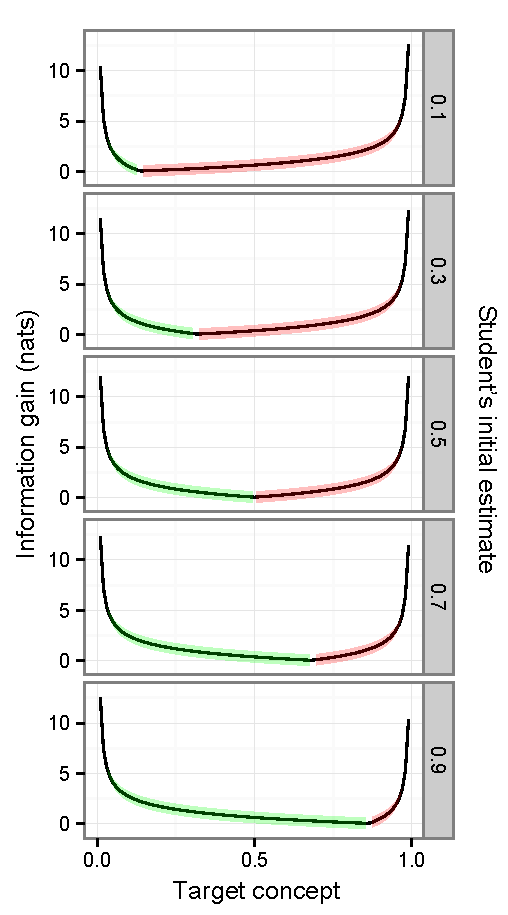
\includegraphics[width=2.5in]{figures/single_student_gain.pdf}
\end{center}
\caption{\label{fig:student} Information gain for the optimal teaching move plotted by teacher's intended concept ($\mu$), for students with different initial starting points. Green highlighting shows ranges in which the teacher's best move is providing a head (0), while red highlighting shows the range where a tail (1) produces greater gain.}
\end{figure}

In our first simulation, we examined the teacher's optimal strategy (and information gain) for a single student. We generated students with biases $\mu= \{.1, .3, .5, .7, .9\}$, and varied the teacher's target concept $C$ smoothly in the interval (0,1). For each combination of $\mu$ and $C$, we assumed that the teacher chose the better of the two possible examples (H or T). 

Results are shown in Figure \ref{fig:student}. Following our intuitions, information gain is greatest when the teacher's concept is extreme, and when the student's initial expectation is mismatched to that concept. In addition, the teacher's optimal strategy (shown by the red or green ribbon) changes depending on the student's initial expectation. Consider the top panel: When the student starts out believing $C=.1$, the teacher should almost always select $T$ as her example, though the relative information gain can be low if the disparity between the student's belief and the teacher's is not large (e.g. if $C=.2$). Note also that information gain can be very slightly negative in the case that the student's belief exactly matches that of the teacher.

\subsection{Student variability}

\begin{figure}[t]
\begin{center}
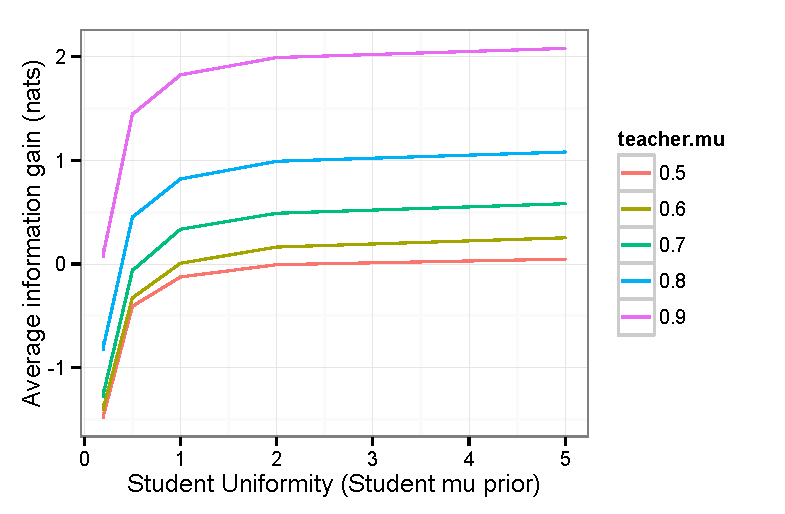
\includegraphics[width=3.5in]{figures/student_uniformity.pdf}
\end{center}
\caption{\label{fig:uniformity} Information gain plotted by the prior on students' uniformity (a symmetric Beta prior on $\mu$ for each student). Target values for $C$ are shown in different colors. Error bars show 95\% confidence intervals.}
\end{figure}

Our next set of simulations combines several students in a single classroom. In these and all subsequent simulations, we generate students randomly via a symmetric Beta prior on $\mu$. With prior values $< 1$, this produces students with extremal biases (e.g. close to 0 and 1), while with prior values $>1$, this produces students whose biases tend to be clustered closer and closer to .5. For each classroom, we assume that the teacher calculates her expected information gain for her two possible strategies and then uses the better of the two. 

Greater student uniformity produced greater information gain, for all target concepts. Figure \ref{fig:uniformity} shows this relationship. The effect was greatest for the smallest values, and information gain was very low when students' expectations tended to be extremal but the target value was closer to the middle of the range. 

For $\mu$ priors $< 1$ information gain can actually be negative; this result comes about when student expectations are extremal but the target value is moderate. In these cases, a single piece of evidence will either reinforce students' biases (in the case that their guess is already close to 1 and they see a $T$) or fail to counteract their biases (in the case that their guess is 0 and they see a $T$). The average of these two cases is negative.

This simulation suggests that a more heterogenous classroom will learn less, on average, because the teacher will be less able to tailor her examples to the students' knowledge. In contrast, in a more homogeneous classroom, the teacher can better provide an example that leads to learning for all students. 

\subsection{Classroom Size}

\begin{figure}[t]
\begin{center}
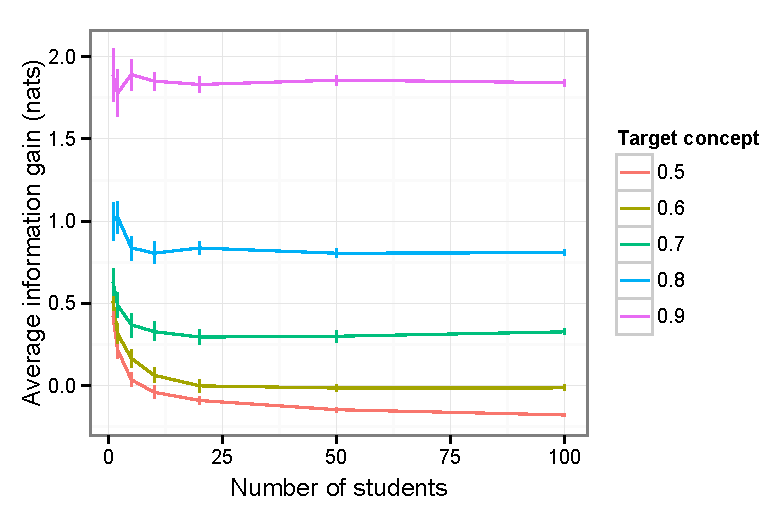
\includegraphics[width=3.5in]{figures/class_size.pdf}
\end{center}
\caption{\label{fig:class} Information gain plotted by the number of students in a class. Target values for $C$ are shown in different colors. Error bars show 95\% confidence intervals.}
\end{figure}

In our next simulation, we examine classroom heterogeneity from a different perspective. As the last simulation set showed, all else being equal, heterogeneity of students is negative relative to the teacher's choice of strategy. More heterogeneous students provide the teacher less of a chance to customize the teaching environment to each student's knowledge state (assuming she knows what that knowledge state is). An important corollary of this finding is that (again, all else being equal) class size is an important factor controlling heterogeneity. Larger classes should be, on average, more heterogeneous, and should hence provide fewer opportunities for teachers to customize their message to the students. 

We created simulated classrooms ranging in size from 1 -- 100 students, across a range of target values for $C$ and found precisely this effect: Larger classrooms showed less average information gain (Figure \ref{fig:class}). This effect was substantially smaller in magnitude than the heterogeneity effects in the preceding simulations---but because students' $\mu$ values were chosen uniformly at random we did not expect to see large effects.

In addition, the class size effect varied substantially with $C$. For $C=.5$ the effect was most pronounced, because (on average) half of the students in each class begin with a lower value of $\mu$, and the other half begin believing it is higher. As the biases of students in the class cancel each other out (e.g. as the classroom average for $\mu$ converges to .5, on average no individual example will teach the class anything. 

Overall, this simulation suggests that in the presence of a heterogeneous population, class size exerts a negative effect on performance. 

\subsection{Tracking Students by Ability}

\begin{figure*}
\begin{center}
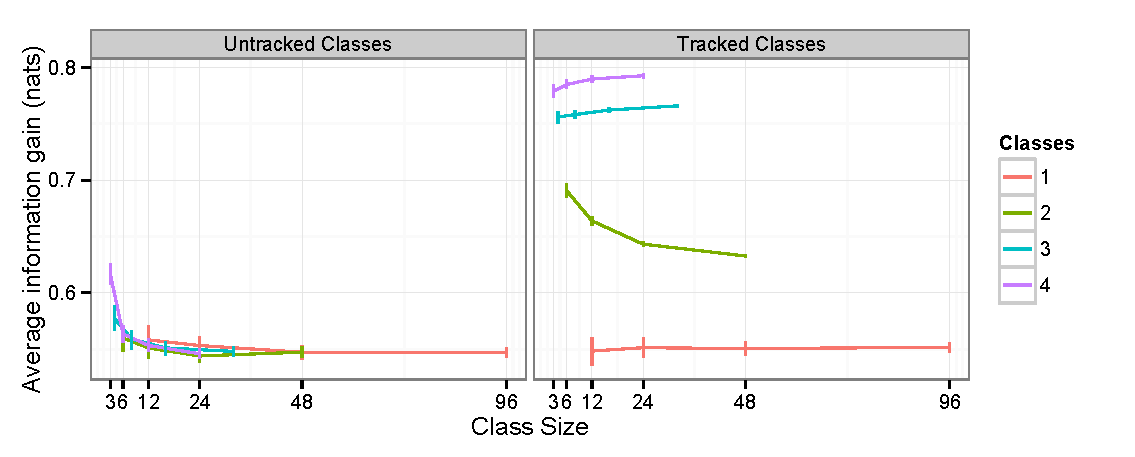
\includegraphics[width=5.5in]{figures/tracking.pdf}
\end{center}
\caption{\label{fig:tracking} Information gain plotted by the number of students in a class. $C$ is set to .75 for illustrative purposes. Colors show the total number of classes among which students were distributed. In the left (untracked) panel, students were distributed at random; in the right (tracked) panel, students were sorted by their prior expectation. Error bars show 95\% confidence intervals.}
\end{figure*}

One way to mitigate class size effects is by reducing classroom heterogeneity. This reduction is sometimes achieved via what is known as ``tracking'': assigning students to classrooms systematically by knowledge or ability, rather than assigning them randomly. In the next simulation, we examine the effects of tracking on classroom performance. 

We created two parallel sets of simulations. In each, a population of students was generated with uniform bias values. The untracked simulations were identical to the class-size simulations above. The tracked simulations were identical except that we sorted students and distributed them into the available classes by their prior knowledge. For example, if there were two classes, the first would receive the students with values of $\mu$ below the median. 

Tracking resulted in greater average information gain for students. Results for an example value of $C$ are shown in Figure \ref{fig:tracking}. While the untracked classes were not differentiated from one another and showed a small class-size effect (left panel), the tracking grew more effective as the number of tracks increased from 2 -- 4. Interestingly, the tracking advantage decreased with each additional group, suggesting that too many tracks created diminishing returns. We also saw no class-size effect for the simulations with 3 and 4 tracking groups: Performance remained stable as size increased, presumably because the classes were homogeneous enough that additional students did not make an appreciable difference to outcomes.  

In our model, class size was a negative predictor of student learning because of the relationship between classroom heterogeneity and student learning. Larger classes tend to be more heterogeneous and hence to have lower performance. Tracking students to more homogeneous classrooms reduced this effect.

\subsection{Mis-tracking for an Individual Student}

\begin{figure}[t]
\begin{center}
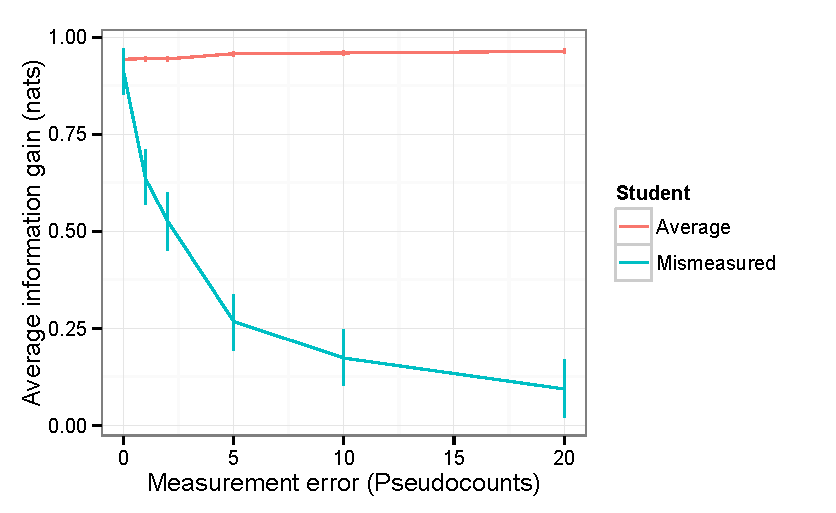
\includegraphics[width=3.5in]{figures/mismeasured.pdf}
\end{center}
\caption{\label{fig:mismeasure} Information gain for the average student (red) and a student whose parameters have been mismeasured (blue), plotted by the error in the measurement. Simulation data are shown for $C=.75$ with four tracked classes of 24 students each. Error bars show 95\% confidence intervals.}
\end{figure}

What happens if you are tracked to the wrong classroom? In our last simulation, we explore the fidelity of the measurement of individual students' competence in the tracking scenario described above. We start with the scenario of a group of students tracked into four classes (shown in Figure \ref{fig:tracking}). 


\section{Discussion}

Class size is an important feature of children's instructional environment. \cite{glass1979}.


\section{Acknowledgments}

Thanks to Noah Goodman, Long Ouyang, and Roger Levy for valuable discussion.

\bibliographystyle{apacite}

\setlength{\bibleftmargin}{.125in}
\setlength{\bibindent}{-\bibleftmargin}

\bibliography{teaching}


\end{document}
